\section{Network Layer}

\subsection{Introduction}

\key{Key Network-Layer Functions}
\begin{figure}[H]
  \centering
  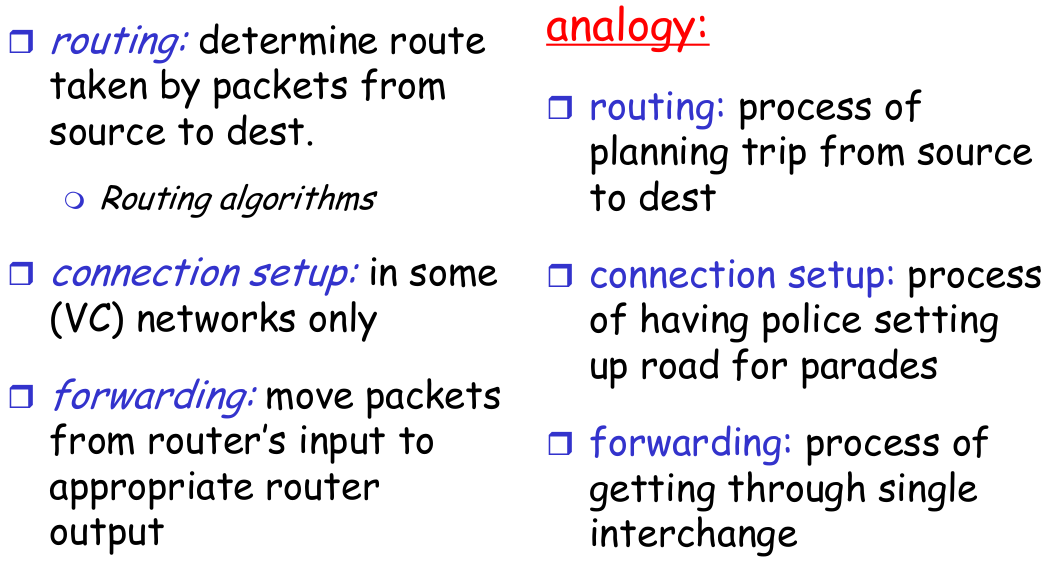
\includegraphics[width=0.48\textwidth]{network_key}
\end{figure}

\subsection{Virtual circuit and datagram networks}

\key{Virtual Circuits vs. Datagram Networks}
\begin{figure}[H]
  \centering
  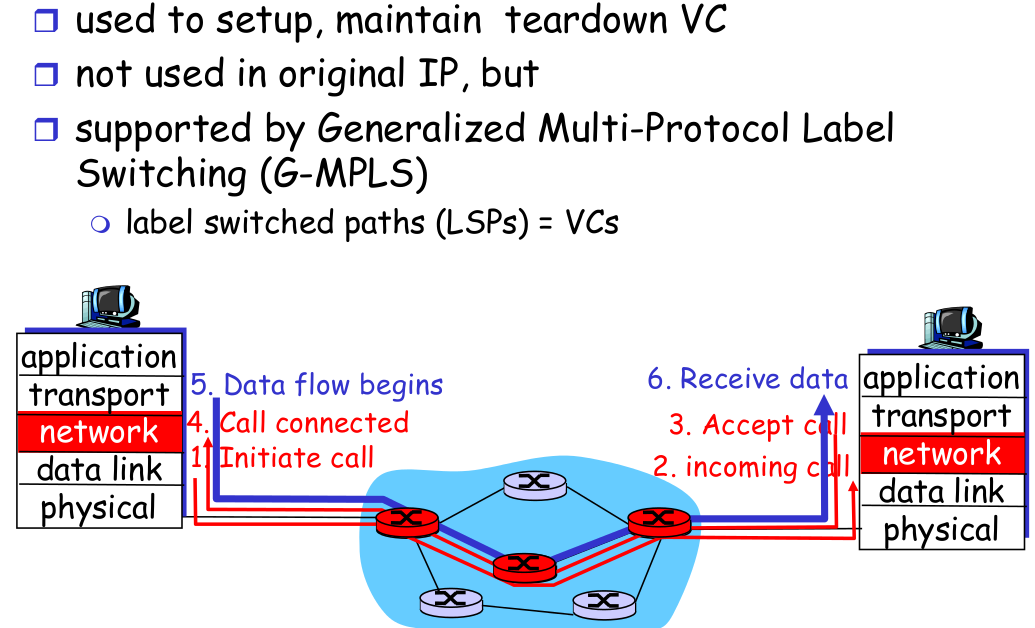
\includegraphics[width=0.48\textwidth]{vc}
  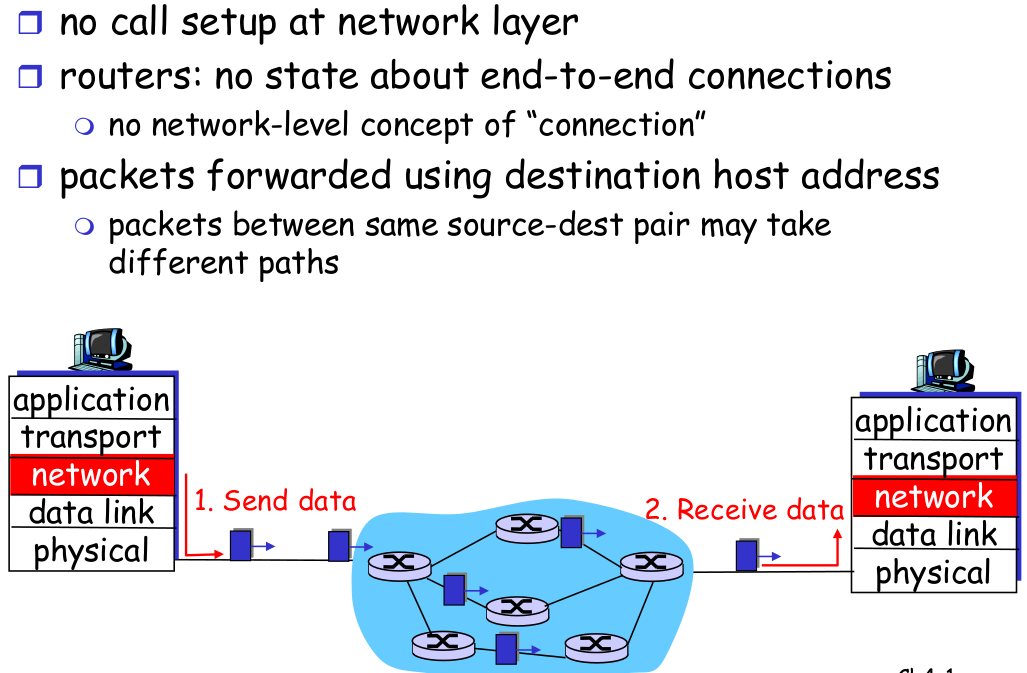
\includegraphics[width=0.48\textwidth]{dg}
\end{figure}

\subsection{IP: Internet Protocol}

\key{IP datagram format}
\begin{figure}[H]
  \centering
  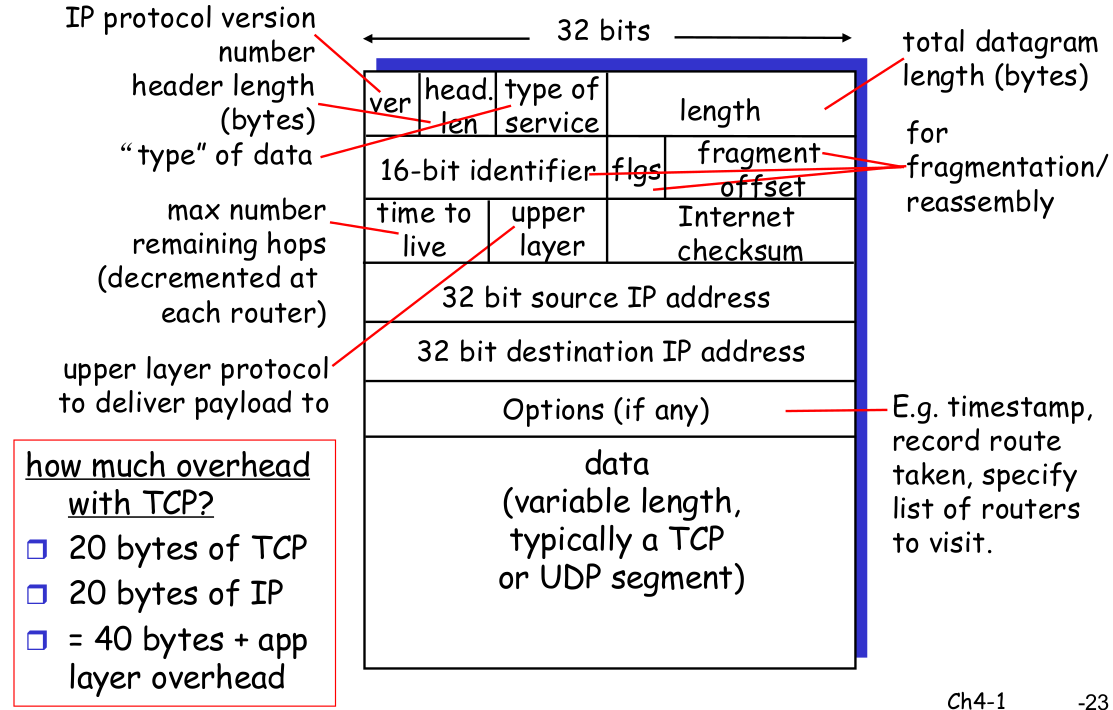
\includegraphics[width=0.48\textwidth]{ip_frame}
  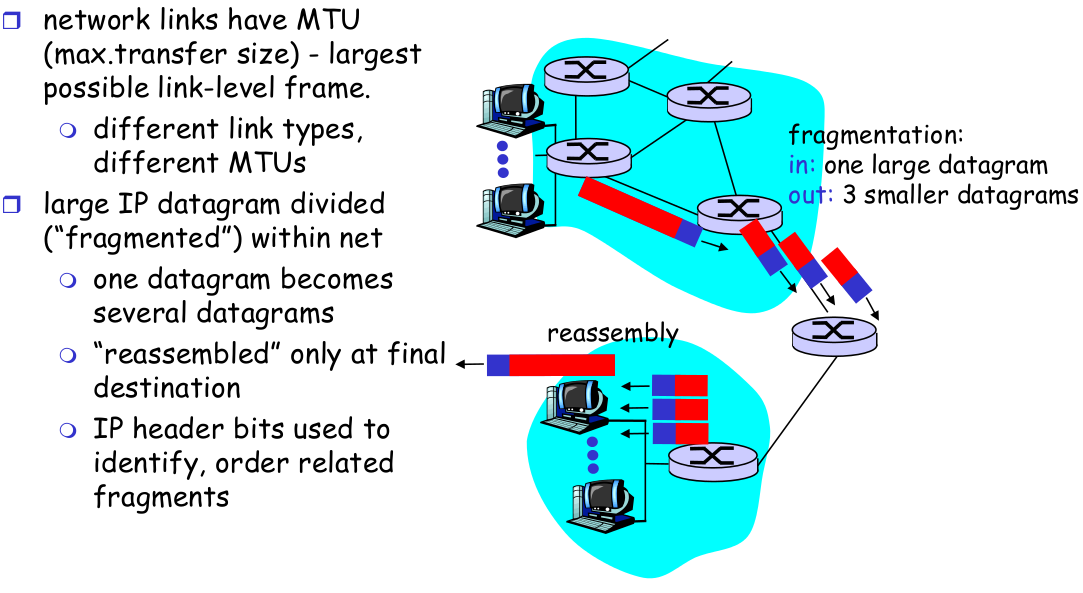
\includegraphics[width=0.48\textwidth]{ip_frag}
\end{figure}

\key{IP addressing: CIDR}
\begin{figure}[H]
  \centering
  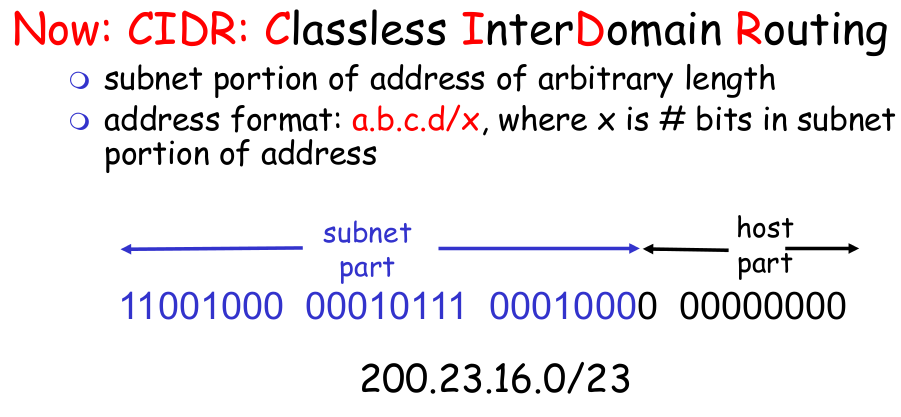
\includegraphics[width=0.5\textwidth]{ip_cidr}
\end{figure}


\key{NAT: Network Address Translation}
\begin{figure}[H]
  \centering
  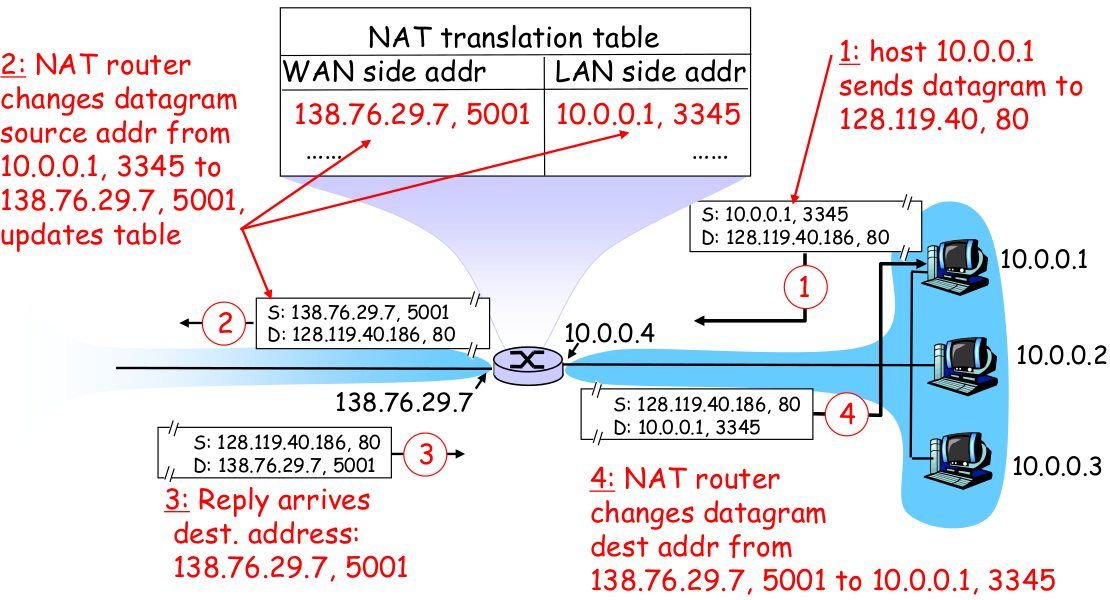
\includegraphics[width=0.48\textwidth]{ip_nat}
  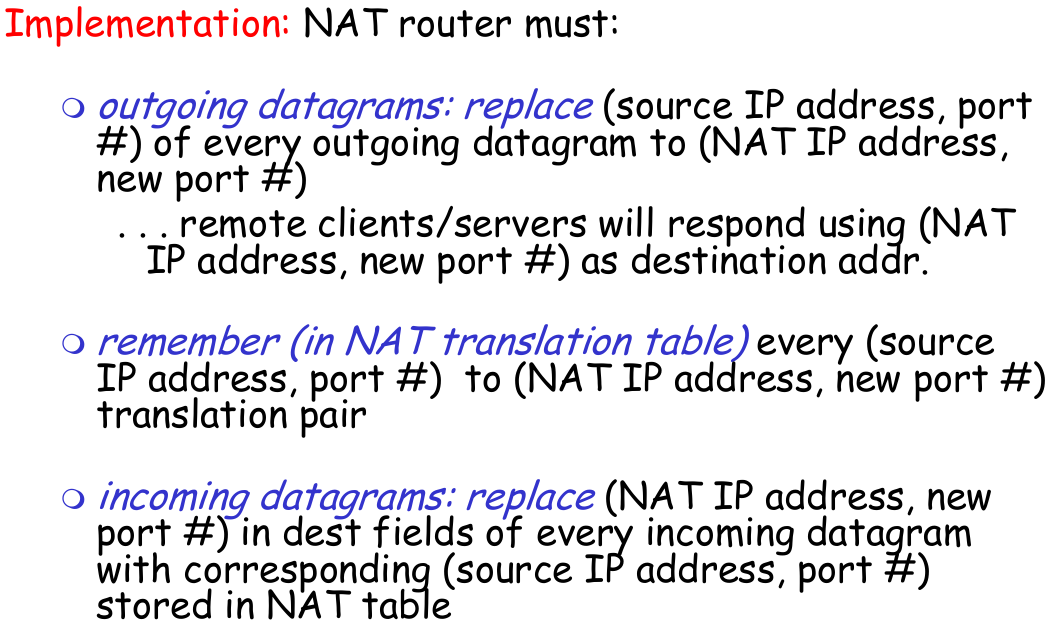
\includegraphics[width=0.48\textwidth]{nat_impl}
\end{figure}

\key{DHCP client-server scenario}
\begin{figure}[H]
  \centering
  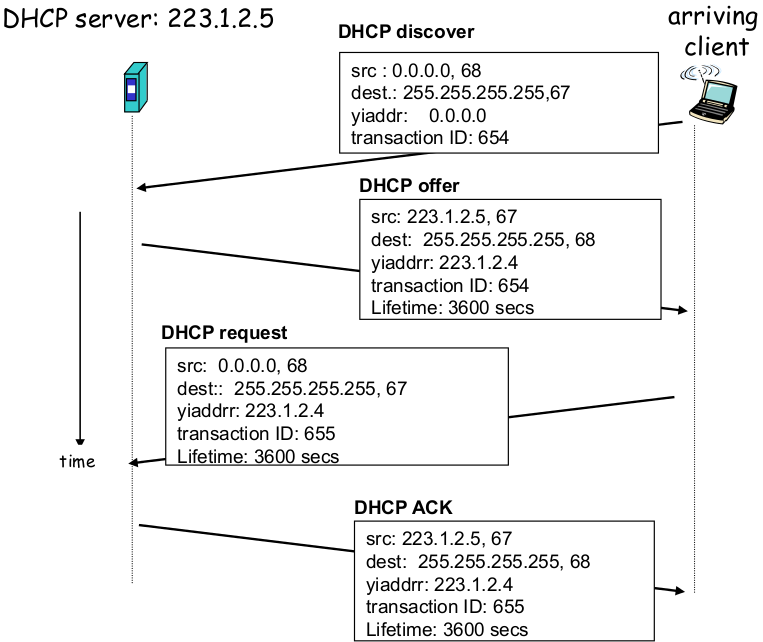
\includegraphics[width=0.48\textwidth]{ip_dhcp}
  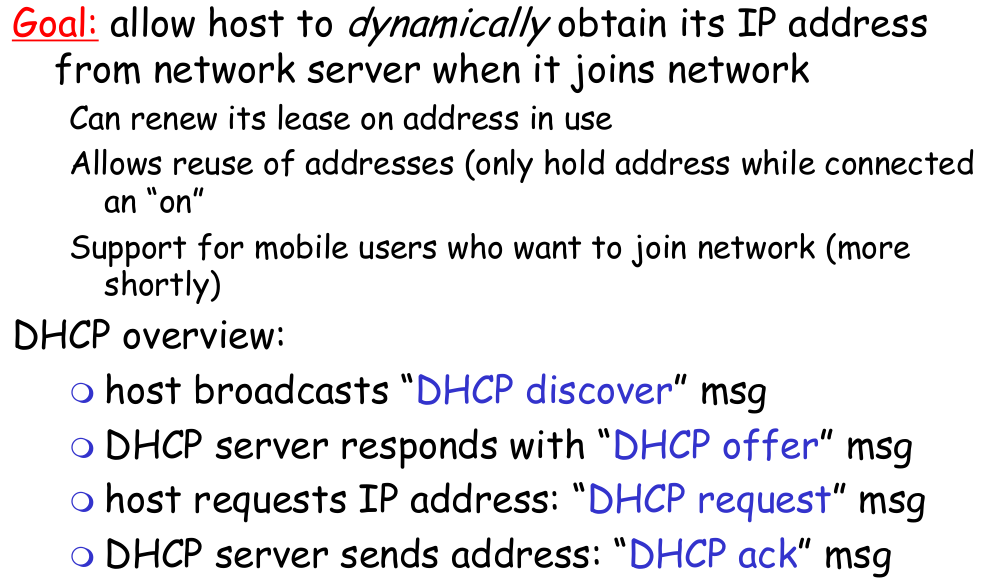
\includegraphics[width=0.48\textwidth]{dhcp_goal}
\end{figure}

Client has to send DHCP request because it probably receive multiple DHCP offers
from different DHCP servers, so that other DHCP servers can know which offer the
client is taking, and can withdraw their offers.

\subsection{Routing algorithms}

\key{Dijkstra algorithm}
\begin{figure}[H]
  \centering
  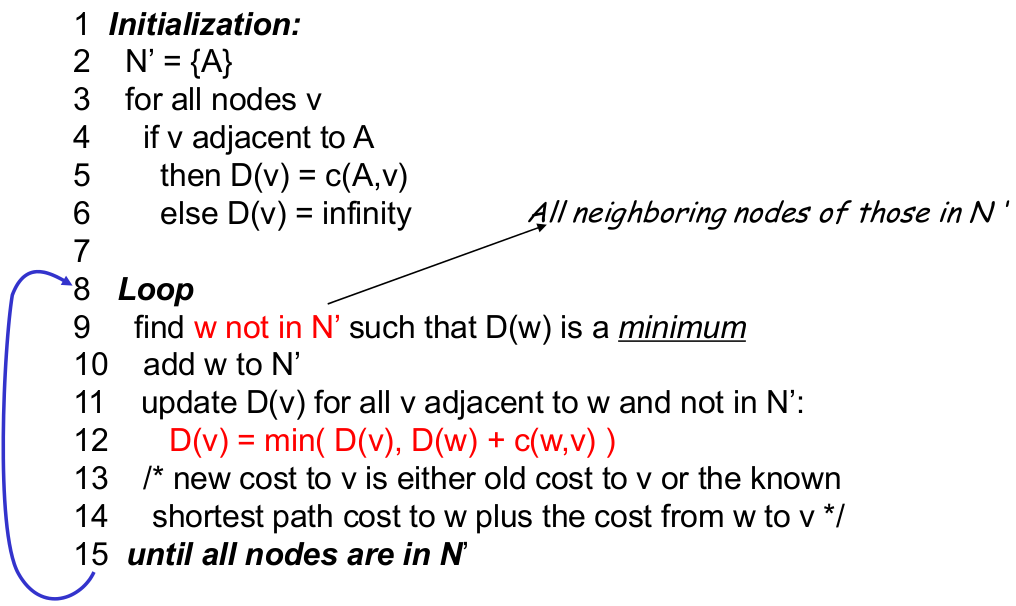
\includegraphics[width=0.49\textwidth]{dijkstra}
  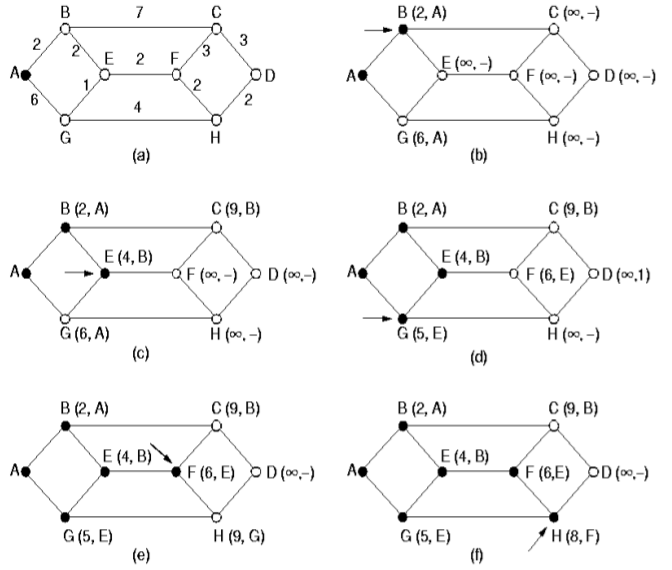
\includegraphics[width=0.49\textwidth]{dijkstra_example}
\end{figure}

\key{Distance Vector}
\begin{figure}[H]
  \centering
  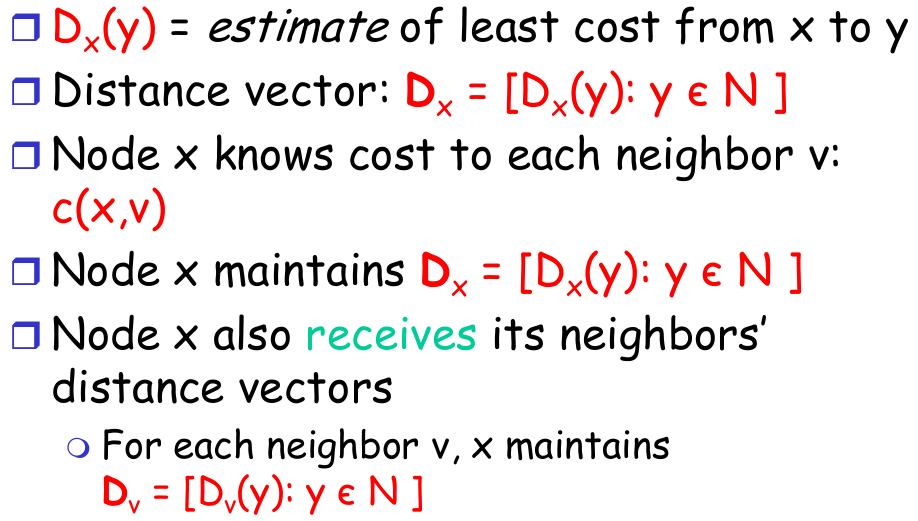
\includegraphics[width=0.49\textwidth]{dv1}
  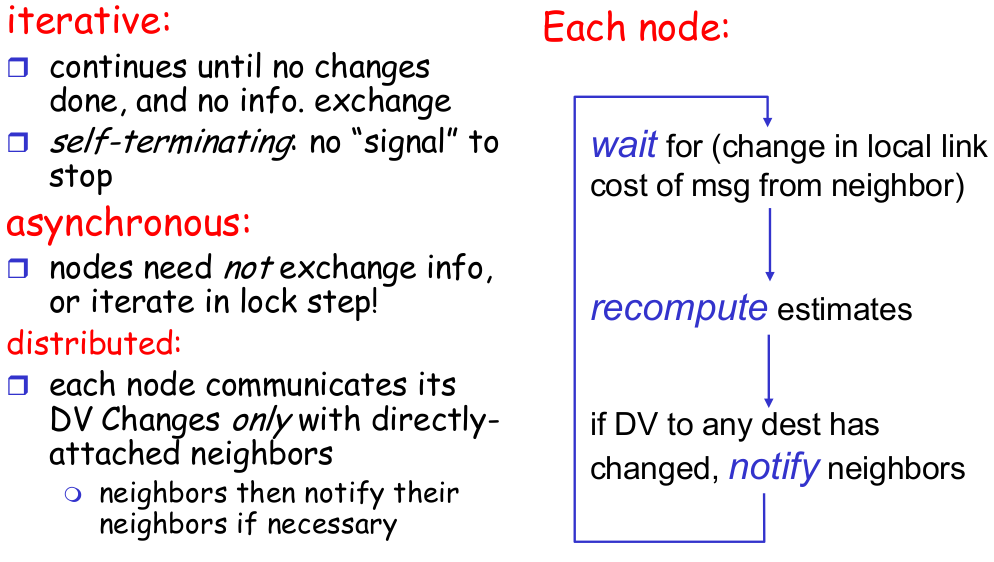
\includegraphics[width=0.49\textwidth]{dv2}
\end{figure}



\key{Hierarchical Routing}
\begin{figure}[H]
  \centering
  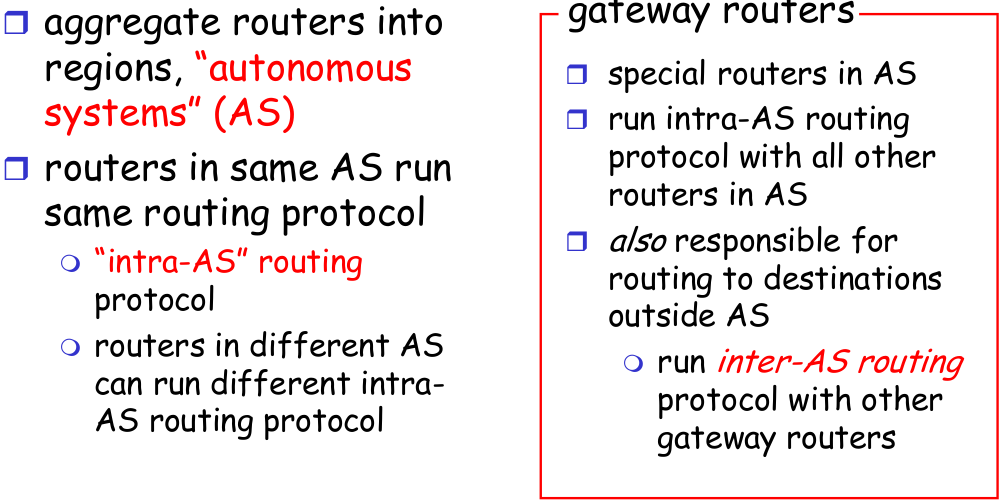
\includegraphics[width=0.5\textwidth]{ip_hierarchy}
\end{figure}

\subsection{Routing in the Internet}

\key{Intra-AS and inter-AS Routing}
\begin{figure}[H]
  \centering
  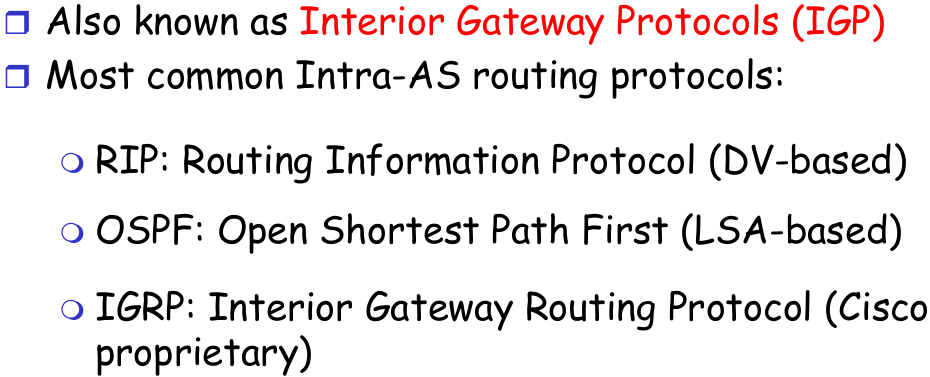
\includegraphics[width=0.49\textwidth]{ip_intra}
  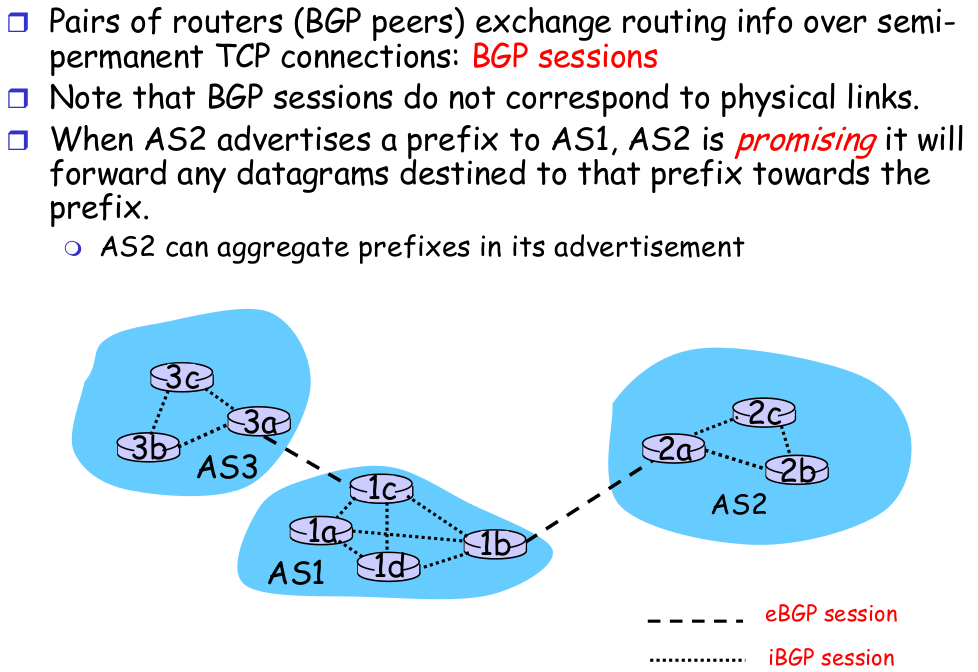
\includegraphics[width=0.49\textwidth]{ip_bgp}
\end{figure}

\key{Why different Intra- and Inter-AS routing ?}
\begin{figure}[H]
  \centering
  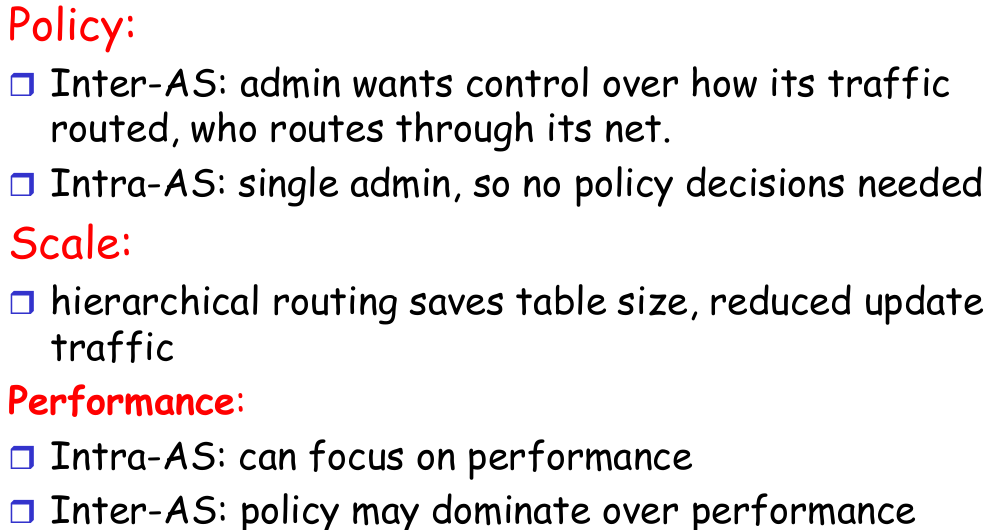
\includegraphics[width=0.5\textwidth]{ip_intra_vs_inter}
\end{figure}

\subsection{Broadcast and multicast routing}

\key{Multicast Routing}
\begin{figure}[H]
  \centering
  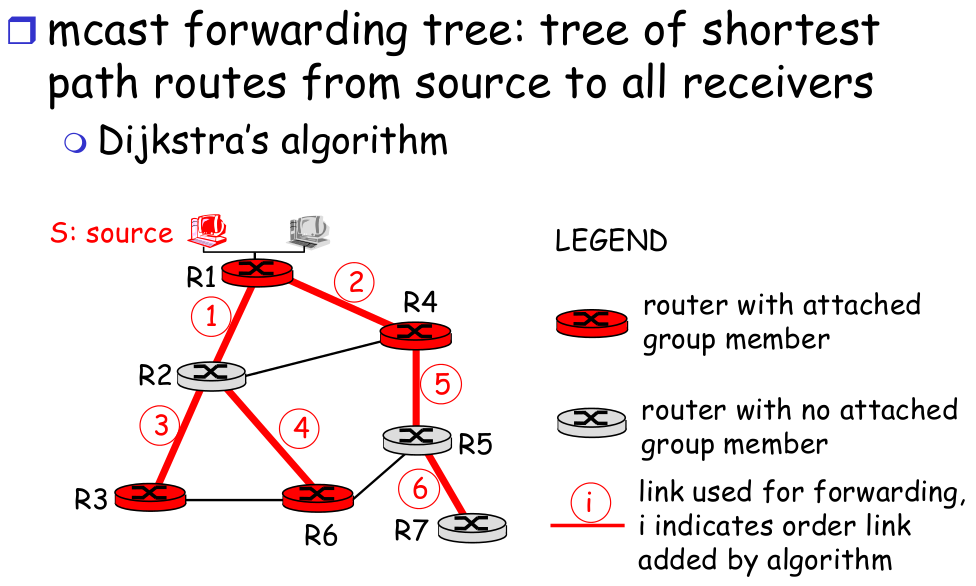
\includegraphics[width=0.49\textwidth]{source_based}
  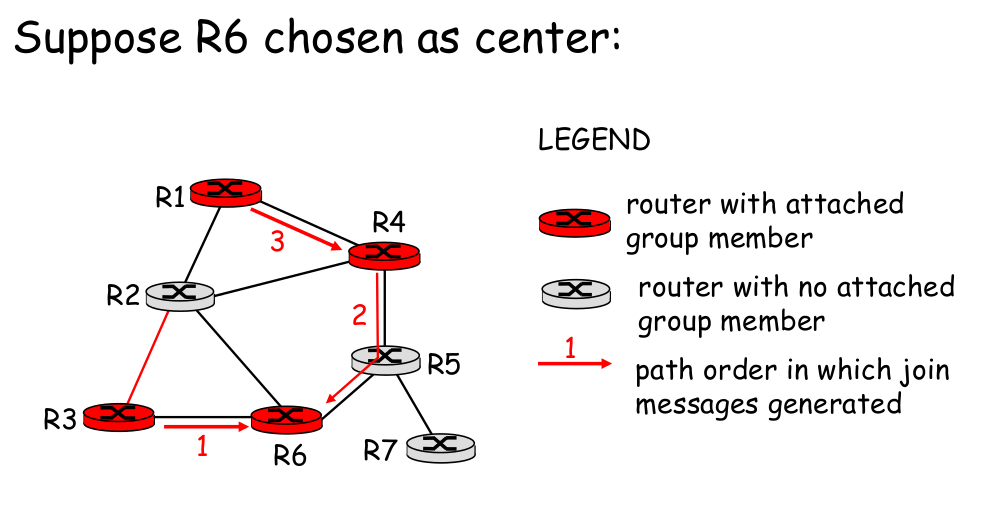
\includegraphics[width=0.49\textwidth]{center_based}
\end{figure}
